\chapter{Introduction}
\label{chap:introduction}

In this work we use the verification framework Stainless to verify parts of the code of Bitcoin-S, a Scala implementation of the Bitcoin protocol.
In the following we describe the main aspects of formal verification, Stainless and Bitcoin-S.


\section{What is formal verification}
\label{sec:formal_verification}

// TODO move to chapter description and change Overview of stainless to formal verification with stainless

The longer and more complex a source code is, the more difficult it is to verify its correctness.
There are different approaches to show the correctness of a program.

A powerful method to check whether a program works correctly is formal verification.
This is a systematic process based on mathematical modeling.
With formal verification all possible inputs are covered algorithmically.
This is in contrast to testing, where only predefined inputs are tested.
The correctness of a program is analyzed relative to its formal specification.
Formal specification is a mathematical description of a software behavior that can be used by the verification tool to verify the code.
We will see an example shortly.

One of such tools is Stainless which we use in our work.


\section{Overview of Stainless}
\label{sec:stainless}

Stainless is developed by "Lab for Automated Reasoning and Analysis" (LARA) at EPFL's School of Computer and Communication Sciences.
Using this framework we can verify the correctness of Scala programs.
Stainless statically verifies that a program satisfies a given specification and that a program will not crash at runtime.
The framework explores all possible inputs and finds a counter examples for possible failures in a program which violate the given specification. \cite{Stainless:introduction}

The main functions used to write a specification are \textit{require} and \textit{ensuring}. 
With \textit{require} we define a precondition of a function, which we want to verify.
\textit{require} is placed at the beginning of the function body.
We pass a constraint for the inputs of a function as an argument to \textit{require} in the form of a Boolean expression.

With \textit{ensuring} we provide a postcondition which is a condition on an output of the function.
\textit{ensuring} is called after the function body.

On invoking, Stainless tries to prove that the postcondition always holds, assuming the given precondition does hold. \cite{Stainless:introduction}

The following example demonstrates a simple formal specification for the function calculating factorial.
This is a modified example from the Stainless documentation, so Stainless reports an error verifying it.
\begin{lstlisting}[language=Scala]
  def factorial(n: Int): Int = {
      require(n >= 0)
      if (n == 0) {
        1
      } else {
        n * factorial(n - 1)
      }
  } ensuring(res => res >= 0)
\end{lstlisting}

The function recursively calculates factorial of an integer number.
The input of the function is constrained with \textit{require} to a non-negative value.
The result should also be non-negative.
Thus, Stainless will verify whether the result of the factorial calculation is non-negative for all non-negative inputs.

Stainless can produce 3 outcomes of postcondition verification: \textit{valid}, \textit{invalid} and \textit{unknown}.
If the postcondition is \textit{valid} Stainless could prove that for any inputs constrained in the precondition, the postcondition always holds.
Reporting the postcondition as \textit{invalid} the framework could find at least one counterexample which satisfies the precondition but violates the postcondition.
If Stainless is unable to prove the postcondition or find a counterexample it reports the outcome \textit{unknown}.
In this case a timeout or an internal error occurred.
Furthermore, Stainless checks for calls in the code to the function with invalid arguments violating the precondition.
For example if we invoke factorial with a negative number it reports \textit{invalid}. \cite{Stainless:introduction}

Let's return back to our incorrect example with factorial.
Stainless reports the following result for the factorial verification from our example:
\begin{figure}[H]
	\centering
		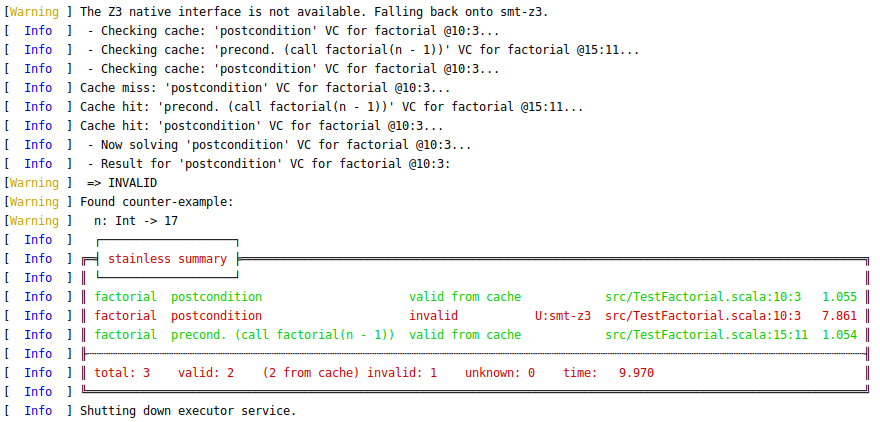
\includegraphics[scale=0.5]{images/output1.png}
	\caption{Output of Stainless verification for calculating factorial of Int number}
	\label{fig:output1}
\end{figure}

Stainless disproves the postcondition and gives the number 17 as a counterexample.
Due to an overflow in the 32 bit Int the result becomes a negative value.
The program would work correct by changing the type from Int to BigInt.

Stainless supports only a subset of Scala.
They call is Pure Scala.
You can find the specification of Pure Scala on the Stainless website\footnote{\url{https://epfl-lara.github.io/stainless/purescala.html}}.

In addition, Stainless has its own library with annotations, reimplementaion of some core data types, collections and input-output functions and more.
Some of them are described on the website\footnote{\url{https://epfl-lara.github.io/stainless/library.html}}.
There are more details about library in the source code of Stainless on GitHub in the folder \textit{frontends/library/stainless}\footnote{\url{https://github.com/epfl-lara/stainless}}.

Stainless verifies Scala programs using SMT (satisfiability modulo theories) solvers. 
The framework transforms a program code to the Pure Scala fragment supported by Inox solver.
This solver was also developed by LARA-Group and allows usage of different SMT solvers such as Z3, CVC4 and Princess, adding support of other higher-level features.
Thus, preconditions, postconditions and assertions are translated into SMT formulas, so an SMT solver can determine if all properties hold.\cite{Stainless:introduction}\cite{Stainless}


\section{Overview of Bitcoin-S}
\label{sec:bitcoin_s}

In the work we verify some fragments of the code of Bitcoin-S.
Bitcoin-S is an open source Scala implementation of the Bitcoin protocol. 
There are different projects belonging to Bitcoin-S.
Protocol data structures are defined in the package \textbf{bitcoin-s-core}.
This package is the main target to be verified because it specifies the base of Bitcoin protocol, and it is crucial for correct protocol functionality.
There is also the package \textbf{bitcoind-rpc} which is an RPC client implementation to communicate with \textit{bitcoind}, daemon of Bitcoin Core running on a machine.
Developers of Bitcoin-S are working on the implementation of a lightweight bitcoin client in the package \textbf{bitcoin-s-spv-node}.
The whole list of packages can be found on GitHub\footnote{\url{https://github.com/bitcoin-s}}.

Bitcoin-S is a large project implementing many functionalities.
In this work one of them is going to be examined and worked on, namely the property of the Bitcoin that a non-coinbase transaction can not generate new coins.
Thus, the code of Bitcoin-S should be analyzed, and fragments implementing this feature should be identified.
Afterwards, the fragments should be rewritten, so that Stainless can accept it.
After that a formal specification for functions should be defined and annotated according Stainless libraries, so that Stainless can verify correctness of the code.


\subsection{No Inflation Property}



\subsection{Addition with Zero Property}


